\documentclass{article}
\usepackage{graphicx}
\usepackage{hyperref}
\usepackage[margin=1.25in]{geometry}
\graphicspath{{pics/}}

\title{50.005 Computer System Engineering}
\author{Shaun Toh, Joel Huang}

\begin{document}
\maketitle

\section{Networking Basics}
\subsection{How to share the Internet}
Packets are a unit of data made out of a header and a payload.\\\\
The internet is a shared resource, so how do we allocate resources, given data traffic is bursty by nature? Packet Switching and Statistical Multiplexing are essentially carried out at the same time on networks. Packets enable accountability, statistical multiplexing allows multiple channels.

\subsubsection{Packet Switching}
Packet Switching is breaking data into blocks instead of a stream.\\\\
Connectionless Packet Switching is when each packet contains the complete address and/or routing information, opening the possibility of an out-of-order delivery and different paths of transmission, while also possibly increasing the speed due to the ability to route packets to network nodes with lower loads.\\\\
Packets contain the following information:
\begin{itemize}
\item Destination address
\item Source Address
\item Total Piece number
\item Sequence number, for reassembly and accounting purposes.
\end{itemize}
Packets are rearranged to form the original message after receiving. This allows for checking of the various packets and requests for re-sending on data corruption or packet loss.\\\\ 
Connection Oriented Packet Switching is very similar, the only difference being the route is predefined, so address information is not sent with the packets. This is also known as virtual circuit switching.\\
\par 

\subsubsection{Multiplexing}
\noindent \textbf{Statistical Multiplexing}\\\\
Statistical Multiplexing is dynamically allocating bandwidth to a channel on a as-needed basis. \\\\
Bandwidth is only allocated to channels that are currently broadcasting as a result, we are able to use multiple communications on the same channel at the same time. Keep in mind that this is a dynamic method, as opposed to the two methods listed below. The main difference is that the sharing is adapted to the current demand, as opposed to a static link sharing method like the next two methods.\\\\

\noindent \textbf{Circuit Switching}
\begin{itemize}
\item \textbf{Frequency Dimension Multiplexing}\\
Frequency Dimension Multiplexing is essentially dividing up total bandwidth in a communication medium into non-overlapping frequency bands. This allows one channel of communication through each band of frequency. \\\\
NOTE: Circuit Switching is a mode of communication where two clients have to establish a dedicated communications channel (a circuit) through the network before any communication can take place. As a result, the full bandwidth of the particular medium is available.

\item \textbf{Time Dimension Multiplexing}\\
Time dimension multiplexing is transmitting and receiving independent signals over the same signal path. While it guarantees complete usage of the entire bandwidth during the period on which this signal is using the line, other signals cannot share the line in the meantime. Instead, all signals take turns using the entire bandwidth. The high speed at which it occurs creates an illusion of concurrency. (While it is effectively concurrent to us).
\end{itemize}

\subsection{Layering}
The same way that making your code in terms of modules and functions enables modularity and easier debugging (you can narrow down the source), Networking is also layered. With each layer implementing only a single service, and only interacting with the layer above and below it, we can narrow down the problem with greater ease. Of note is that Network Layering results in cascaded headers. i.e. Every layer just adds their own header to the packet that is being sent.\\

\subsubsection{The Internet Protocol Stack}
The Internet protocols are layered as follows:\\
\begin{itemize}
\item \textbf{Application Layer Protocols:} Supporting network Applications: FTP, SMTP, HTTP
\item \textbf{Transport: Process-process data transfer:} TCP, UDP
\item \textbf{Network:} Routing of datagrams from Source to destinations -IP, Routing protocols
\item \textbf{Link:} Data transfer between neighbouring network elements: Ethernet, 802.11 (WiFi), PPP
\item \textbf{Physical:} Bits "On the Wire"
\end{itemize}

\subsection{Host to Host Layer Protocols}
\subsubsection{UDP}\\
The User Datagram Protocol is lightweight compared to TCP. It doesn't require reliable delivery and extra overhead, so reliability is outsourced to the application layer. \textbf{Real time traffic} utilizes this protocol as it cares only about fast transmission. UDP packets have a header of 8 bytes (64 bits):\\\\
\begin{center}
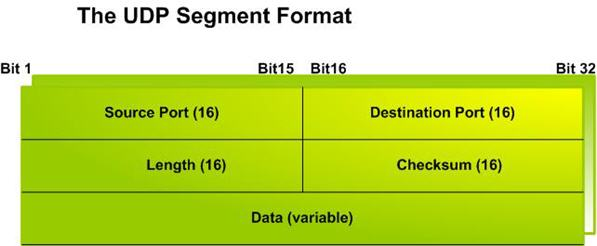
\includegraphics[width=\textwidth]{UDP.jpg}\\
\url{<https://www.pluralsight.com/blog/it-ops/networking-basics-tcp-udp-tcpip-osi-models>}\\
\end{center}
\pagebreak

\subsubsection{TCP}
TCP stands for Transmission Control Protocol. It is known to be connection oriented. This is because both parties have to establish a connection before beginning to transmit data. TCP communicates via segments of data, consisting of a fixed 20 byte header and a variable size data field at the end. Of note is the \textbf{constant back and forth of acknowledgement} requests from both machines. This protocol is hence able to maintain and ensure integrity of data sent and received.\\\\
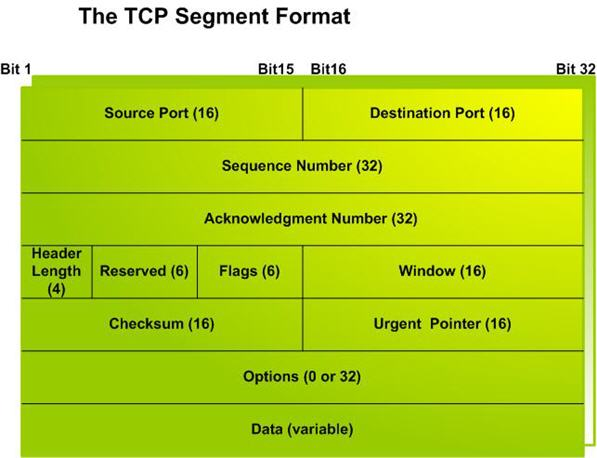
\includegraphics[width=\textwidth]{TCP.jpg} \\
\url{<https://www.pluralsight.com/blog/it-ops/networking-basics-tcp-udp-tcpip-osi-models>}\\

\begin{itemize}
\item \textbf{Source Port} and \textbf{Destination Port} fields together identify the two local end points of the particular connection. A port plus its hosts' IP address forms a unique end point. Ports are used to communicate with the upper layer and distinguish different application sessions on the host.
\item The \textbf{Sequence Number} and \textbf{Acknowledgment Number} fields specify bytes in the byte stream. The sequence number is used for segment differentiation and is useful for reordering or re-transmitting lost segments. The Acknowledgment number is set to the next segment expected.
\item \textbf{Data offset} or TCP header length indicates how many 4-byte words are contained in the TCP header.
\item The \textbf{Window} field indicates how many bytes can be transmitted before an acknowledgment is received.
\item The \textbf{Checksum} field is used to provide extra reliability and security to the TCP segment by detecting changes in the header and data content. IPv4 and IPv6 use different methods to compute the checksum.
\item The actual \textbf{Data} is included after the end of the header. \\
\end{itemize}

\subsubsection{Internet Control Message Protocol}
The Internet Control Message Protocol (ICMP) is a supporting protocol, generally used for sending error messages or operational information. It is not typically used to transmit data and is utilised by \textbf{Ping} and \textbf{Traceroute}. Both end hosts and routers utilise this protocol. It is not the same as other transport protocols such as UDP or TCP. \\

\subsubsection{General comparison between TCP and UDP}
\begin{center}
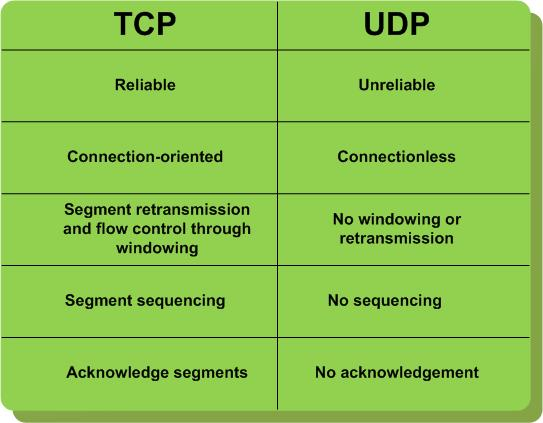
\includegraphics[width=\textwidth]{TCPUDPComparison.jpg} \\
\url{<https://www.pluralsight.com/blog/it-ops/networking-basics-tcp-udp-tcpip-osi-models>}\\
\end{center}
\pagebreak

\subsection{Application Layer Protocols}
Application layer protocols define how applications running on different end systems, process and pass messages to each other. The Application Layer Protocols determine the following aspects:
\begin{itemize}
\item The types of messages, e.g., request messages and response messages.
\item The syntax of the various message types, i.e., the fields in the message and how the fields are delineated.
\item The semantics of the fields, i.e., the meaning of the information that the field is supposed to contain.
\item Rules for determining when and how a process sends messages and responds to messages.
\end{itemize}
Applications adhere by these rules allowing for a universal standard of communication. There are a few application protocols that are highlighted in this course.

\subsubsection{HTTP (TCP)}
HyperText Transfer Protocol (HTTP) defaults to port 80. It utilizes TCP connections to send client requests and server replies.

\subsubsection{FTP (TCP/UDP)}
File Transfer Protocol establishes 2 connections between hosts. It uses one connection for control, and another for data. As a result of the absolute separation, it is able to transfer data more reliably and efficiently. FTP is able to handle binary and .txt formats.

\subsubsection{SMTP (TCP)}
Simple Mail Transfer Protocol is used for emails. It provides services for mail exchange between users on the same or different computers. It is based off a client-server model. Both clients and servers will run this protocol. If you send mail, you act as a client. Receiving mail means you act as a server.

\subsection{Internet Structure}
The internet is essentially a network of networks. Every internet service provider (ISP) is essentially linked together by Internet Exchange Points (IXP). Regional networks might also arise in order to connect access nets to ISPs, while content providers also can create their own networks allowing them to pass data to the internet while bypassing regional ISPs or even international ISPs. To make things clear:

\begin{center}
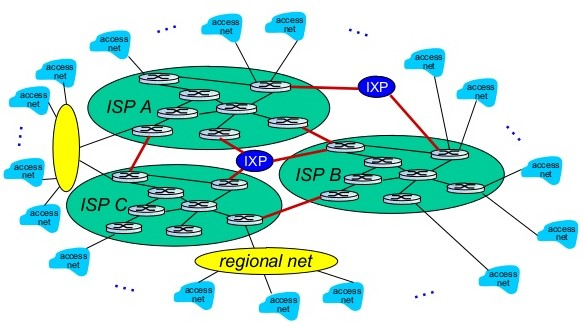
\includegraphics[width=\textwidth]{ISPtiers.jpg}
\end{center}

\begin{itemize}
\item Tier 1: Commercial ISPs (Starhub, AT\&T etc.), Content provider Networks (Google). Essentially the largest global ISPs, as they represent national and international coverage.
\item Tier 2: IXPs. I.e. Connectors between the Tier 1 ISPs.
\item Tier 3: Regional ISPs: Local internet service providers.
\item Tier 4: Local Access Networks (your wires)
\end{itemize}

\section{Network Performance}
\subsection{Sources of delay}

\begin{center}
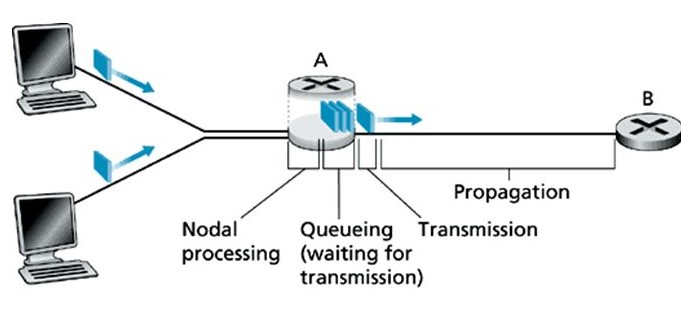
\includegraphics[width=\textwidth]{delays.jpg}
\end{center}

\subsubsection{Transmission delay}
Transmission delay is the \textbf{amount of time it takes for a packet to be sent to the router's outward link}, or back.

\subsubsection{Propagation delay}
Propagation delay is the \textbf{total time the packet spends in transit}. It is influenced by distance from the target destination (or next where the next hop is) and hardware along the link.

\subsubsection{Processing delay}
Processing delay occurs as a result of \textbf{devices processing/examining the packets}. This is unavoidable and can only be reduced by getting better processing components on those devices.

\subsubsection{Queuing delay}
Queuing delay is the \textbf{waiting time for a packet to get to the front of the queue} for the output link. Depending on current traffic and the congestion level of the router, the queuing delay might be very high.

\paragraph{Calculating queuing delay}
R: Link bandwidth (KB/s)\\
L: Packet Length (bits)\\
A: Average packet arrival rate (packets/s)\\
LA/R is the average link utilization and ranges from [0,1]\\
LA/R ~0, there is a small average queue delay.\\
LA/R ~1: There is a large average queue delay \\
LA/R >1: There is more work arriving to the server, skewing the calculations.

\begin{center}
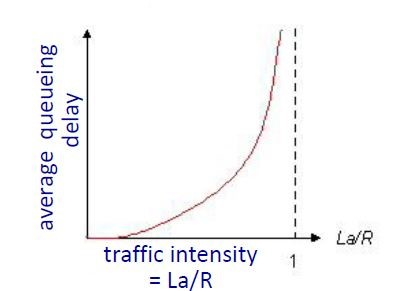
\includegraphics[width=\textwidth]{QueueDelayGraph.JPG}
The queuing delay is a convex increasing function. This means overloading the router will drastically increase queuing delay.
\end{center}


\subsection{Traceroute, Ping, Internet Control Message Protocol}

\subsubsection{Ping}
Ping is a network administration utility tool used to \textbf{test the reachability} of a host on an Internet Protocol (IP) Network. Ping uses the ICMP echo request/reply to messages to check for errors, packet loss, and the maximum and mean roundtrip times (RTT).

\begin{center}
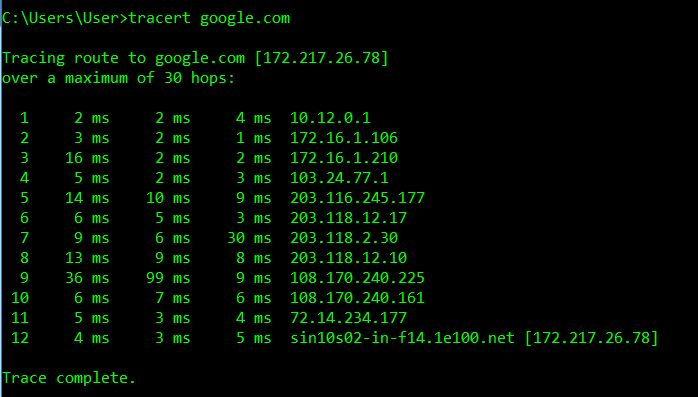
\includegraphics[width=\textwidth]{tracertexample.JPG}
Example of a traceroute (tracert) run on a windows OS. 
\end{center}

\subsubsection{Traceroute (tracert on Windows)}
Traceroute is a network diagnostic tool which \textbf{displays the path that a packet takes} across an Internet Protocol Network. It also records transit delays of packets. The round-trip times of the packets is received from each successive host in the route and the sum of the mean times in each hop is used to measure the complete time spent.

\begin{center}
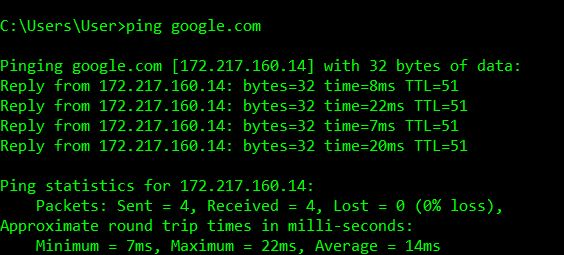
\includegraphics[width=\textwidth]{PingExample.JPG}
Example of a ping command run on a windows OS.
\end{center}

\subsection{Packet Loss and Handling}
The queue within a router has a finite capacity. \textbf{A packet is dropped upon arriving to a full queue, resulting in loss}. Loss can also occur as a result of the link between devices. Loss is ultimately random, and different types of links and congestion situations affect the probability for each link/router. Packet loss is handled by re-transmission from the source end system (TCP), or not at all (UDP). In your calculation of total loss rate, it is important to remember that every pipe works with a different percentage of the packet, i.e., If Pipe 1 loses 5\% of the packet, then Pipe 2, which follows after will only have 95\% of the packets to work with. Therefore, if Pipe 2 had a loss rate of 10\%, it would end up losing 9.5\% of the total packets that were transmitted from your original machine. So the receiving end after pipe 2 would have 0.95 * 0.9 = 85.5\% of the packet. The loss rate can interact with the delay. Depending on whether re-transmission takes place, you can reduce the loss rate, but increase the delay, or do the exact opposite.

\subsection{Throughput}
Throughput (usually KB/s) is the rate at which bits are transferred between senders and receivers. It is important to recognize how throughput is organized throughout a system to identify bottlenecks and optimal paths, as links with lower throughput rate will act as an artificial limit to connection speed.

\subsubsection{Space Time Diagram}
Just for you to know as you may be required to draw it. No Google won't let you find this easily. Again, $L$ is the \textbf{packet length (bits)}, and $R$ is the \textbf{link bandwidth (bits/s)}. 

\begin{center}
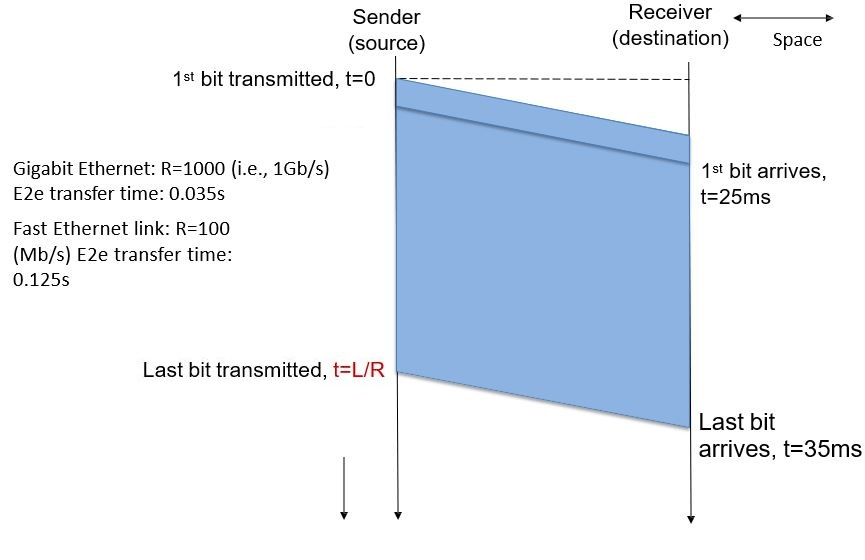
\includegraphics[width=\textwidth]{spacetimediagram.JPG}
\end{center}

\section{Network Security}
General goals in security:
\begin{enumerate}
    \item confidentiality: Limited to intended recipient
    \item authentication: Verification of identities
    \item message integrity: Ensure message is not altered without detection
    \item access and availability: accessible and available to all users
\end{enumerate}

Possible attacks by intruders
\begin{enumerate}
    \item eavesdrop on messages sent
    \item insertion of messages into connection
    \item impersonation of either party (IP Spoofing)
    \item hijacking ongoing connection, taking place of a party
    \item denial of service (DDOS, resource overloading)
\end{enumerate}
\pagebreak
\subsection{Cryptography basics}
Cryptography is the practice or study of techniques for secure communication. It aims to fulfill the goals of security above while preventing attacks. In network security, the basic idea is a function(mechanism) and a number (key) that allows for the obfuscation of information as required. The obfuscated information can then be sent over multiple networks before reaching its intended destination and decrypted. The system relies on the fact that knowledge of the system itself is insufficient to decrypt messages. One also needs to know a unique "key". There are two methods of doing this.
\subsubsection{One-way Functions}
A one way function is also known as a trapdoor function. In order to utilise this kind of method, two numbers are required for the trapdoor function to operate. The first number is used in encryption, but cannot be used for decryption. The second number is the exact opposite, designed only for use in decryption.
\subsubsection{Symmetric Key}
A Symmetric key is based on the idea of a typical mechanical lock. The same key is used both in decryption and encryption.
\subsection{Symmetric Key Encryption}
Symmetric Key encryption involves the following: \\
Where\\
m = message\\
c = Ciphertext\\
KS() = Encryption/Decryption function\\
KS(m) = c\\
m = KS(c)\\
Therefore, before sending confidential information, both parties have to encrypt the message using the encryption function, and then decrypt the message using the same function. However, this raises the problem of sharing the key to begin with.
\subsubsection{Simple Encryption Schemes}
A few examples of simple encryption schemes are:
\begin{enumerate}
    \item ROT1 (Replace every letter with the letter that follows it)\\
    Basically replace A with B, B with C and so on. Prevents prying eyes, but is easily decrypted.
    \item Transposition ciphers (replace every letter with another agreed letter.) \\
    More difficult to decrypt but still easily brute forced, especially with the introduction of computers.
    Of note is how the encryption key only maps from a set of 26 letters to 26 letters. This means that knowledge of a word such as "POP" will result in an easier time decrypting the message via brute force. 
    \item DES (Data Encryption Standard)
    DES is known as a block cipher. It takes a fixed-length string and transforms it through a series of complicated operations into ciphertext of the same length. In the case of DES, the block size is 64 bits. DES also uses a key to customize the transformation, so that decryption can supposedly only be performed by those who know the particular key used to encrypt. The key is composed of 64 bits, 8 of which are used solely for checking parity. Hence the effective key length is 56 bits. It isn't used widely anymore due to its key length being too short.
\end{enumerate}
\subsubsection{Advanced Encryption Schemes}
\textbf{Advanced Encryption Standard}\\
The advanced encryption standard has replaced DES since 2001, processing data in blocks of 16 bytes. Most implementations will chop blocks into sizes of 16 bytes for AES to process. If the block is not sufficient in length to reach 16 bytes, it is padded depending on the chosen padding scheme. Otherwise, a block of 16 bytes is added to the end of the entire cipher text.\\
\textbf{Public Key Cryptography (RSA)}\\
RSA is a system which utilises one-way functions. By using two prime numbers and an auxiliary value, one can create two keys, one of which is known as the public key, and the other, the private key. The public key can be sent to any party on the internet who wishes to send the owner of the keys anything confidential. The system works on the premise that given one of the keys, it should be very difficult for anyone to compute the other key. Some example uses:\\
\begin{itemize}

\item Basic Message sending
\begin{enumerate}
    \item One of the keys is used to encrypt a message, the ciphertext is sent to the intended recipient.
    \item The intended recipient receives the message, and uses the other key to decrypt the message, successfully receiving it.
\end{enumerate}
Of note is that this method is used mainly by other recipients who wish to send private items over to the key owner. They will use the public key to encrypt the message, while the owner uses a private key.

\item Authentication
\begin{enumerate}
    \item In order to authenticate the other user, the server can send an encrypted message using the public key to the user. The message is normally an arbitrary number, known as a nonce.
    \item The user receives the message, and uses the other key to decrypt the message, successfully receiving it, and echoes the encrypted message back to the server, proving that he is indeed the owner of the private key/public key key set that was used. 
\end{enumerate}

\end{itemize}

\par
\subsection{Creating an RSA Key pair}
Just some basic math in case they need it.\\

\begin{enumerate}
    \item choose two large prime numbers
    \item compute a number N = p*q , and another number k = (p-1)*(q-1)
    \item choose e (with e lesser then n) that has no common factors with k.\\
    i.e. relatively prime numbers
    \item choose one more number, C, such that (e*C)-1 is exactly divisible by k
    \item the public key is hence (N,e), and private key, (N,C)\\
\end{enumerate}

\subsection{RSA Encryption and Decryption}

Given the public and private keys,\\
\[Encrypted Message = m^e \bmod N\]\\
\[Decrypted Message = (Encrypted Message)^C \bmod N\]\\
Of note:\\
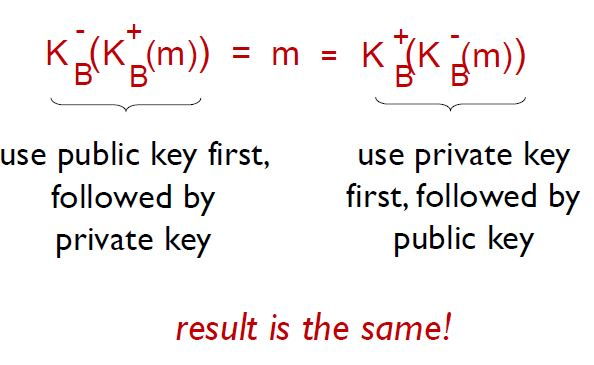
\includegraphics{RSAencryptdecrypt.JPG}\\

\subsection{RSA and AES used in tandem}
RSA is relatively secure, but is extremely slow compared to AES. This is especially due to the computational cost of exponentiation. Therefore, RSA is normally first used for verification purposes, then an AES symmetric key is generated and sent over, allowing for faster and secure communication between both computers.
\subsection{Non-repudiation, and digital signatures}
Digital signatures serve the same function as signatures we make when cashing in our non-existent cheques. Essentially, the signatures are done by encrypting the message with the person's private key. The sender who signs a document establishes that he is the sole creator of the message. A simple example is using RSA encryption to "sign" a message. Because the public key can be used to verify that the message is decryptable, we can verify the owner of the message is the owner of the public key.
\subsection{Message digests}
As it is computationally expensive to public-key-encrypt long messages, hash functions are used to get a fixed, easy to compute digital fingerprint. Collisions are possible in the hash function, but are relatively rare. The point of the message digest is to allow for an easily identifiable fingerprint, allowing for checking if the message was tampered with in transit. Examples of hash functions are SHA-1 or MD5.
\subsection{Certification Authorities}
Given that everyone can generate a certificate, there is nothing stopping anyone from simply stating that they are someone else, while proving that they are owners of the certificate sent over. As a result, certifying authorities serve to verify that public keys are bound to particular entity. Certifying authorities can be government backed or well known service provider.

\section{Internet Naming and Addressing}
\subsection{Further on the DNS: Domain Name System}
The Domain System is a distributed database, implemented in hierarchy of many name servers.\\
Hosts and name servers communicate to resolve names and IP addresses.
\subsubsection{DNS Services}
\begin{itemize}
    \item hostname to IP address translation
    \item host aliasing - canonical, alias names
    \item mail serving aliasing
    \item load distribution (replicated webservers can be used, meaning many IP addresses correspond to one name)
\end{itemize}
\subsubsection{reasons against DNS centralisation}
\begin{itemize}
    \item Single failure point
    \item No way to effectively scale the structure
    \item Traffic Volume (bottleneck)
    \item distant centralised database can result in increased latency
    \item maintenance is difficult
\end{itemize}

\subsubsection{DNS-(UDP type connection)}
Domain Name System is a UDP connection. DNS servers (since they use UDP) don't have keep alive connections, and requests are small and fit well within UDP segments. The TCP/IP protocol uses the IP address of a machine, allowing for unique identification of the connection of a host to the internet. Using a hierarchy of name servers, we are able to resolve Internet host names into the correct IP addresses by issuing a DNS query to the right name server. DNS also allows for mapping of the names to the addresses, allowing humans to navigate the internet using URLs. The DNS hierarchy is structured like this:

\begin{center}
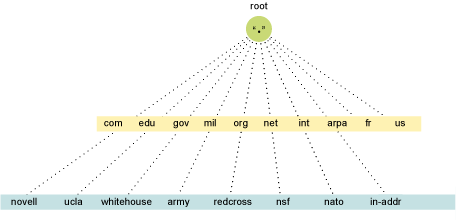
\includegraphics[width=\textwidth]{dns.png}
\end{center}

\begin{itemize}
\item Root.
\item Generic top-level domains (gTLDs), which defines registered hosts according to their generic behaviour, e.g.\{com, edu, goc, mil, net, org\}. Also includes country-code top-level domains (ccTLDs), which define registered hosts according to their country, using 2 character country abbreviations instead of 3 like the generic domain, e.g. \{us, sg, ai\}.
\item The inverse domain, which is used to map an address to a name.
\end{itemize}
\subsection{Basic DNS mechanism}
\begin{enumerate}
    \item Clients requesting web pages query their local DNS server for the appropriate IP address.
    \item If the call was \textbf{recursive} and the server does not have the appropriate answer, the server queries the root DNS servers to find an appropriate DNS server, and continuously makes calls until it manages to obtain the mapping for the requested address. At which point the server then returns the answer to the computer that requested it.
    \item If the call was \textbf{iterative}, the server returns that it has no answer, and the local DNS server then queries the root DNS server, who further directs them to the next correct DNS server in the hierarchy to get the appropriate IP address for the website. (Root servers do not offer recursive call support!)
    \item Upon obtaining the correct IP address, the response is returned to the original requester.
\end{enumerate}
Of Note is that recursive queries are \textit{are not always supported by the server}. This means that it is up to the DNS server to decide if it wishes to pursue the recursive query. This is because recursive queries are burdensome on name servers. If not, the server will only return a reference to another server that the local DNS server/computer can check with to answer the query.
\subsection{Local DNS Servers}
\begin{itemize}
    \item Caches information for local clients requests after retrieving the appropriate answer from an authoritative name server.
    \item Speeds up queries by preventing repeat queries from being requested from the server. \item Past query results are stored for a limited amount of time, known as the TTL (Time to live).
    \item Of note is that cached entries might be out of date. So TTL is important in ensuring a balance between updating cached answers and maintaining efficiency.
\end{itemize}
\subsection{Authoritative servers}
\begin{itemize}
    \item Organization's own DNS server(s), providing authoritative host name to IP for organisation's named hosts.
    \item Is generally maintained by either the organisation or the service provider.
\end{itemize}
\subsection{DNS Server response format}
DNS responses come in a predetermined format with several types of information, depending on the type of information required about a domain.
\subsubsection{Format field}
DNS Servers will reply to queries in a predetermined format. 
\begin{itemize}
    \item Domain Name: The domain name for which the query was sent
    \item Specifies the type of data included in the record
    \item Class: Specifies the data's class. This will be elaborated below
    \item Time to live the number of seconds this record will still be cached. It will be deleted upon expiry
    \item Data Length: Specifies the count of octets in the resource data field
    \item Resource Data: Contains the results of the binding data
\end{itemize}
This format is repeated for all 3 sections of the response. The answer section, Authoritative Name servers section, and the Additional Records Sections.
\subsubsection{Field Types}
\begin{enumerate}
    \item A: this refers to the host address
    \item CNAME: Canonical Name (alias) refers to an alias for eg. www
    \item HINFO: Name of the CPU and Operating System
    \item MINFO: Information on a mailing list or mailbox.
    \item MX: 16-bit preference and name of the host that acts as a mail exchange server for a domain
    \item NS: The authoritative name server for the domain, and its hostname
    \item PTR: Symbolic link for a domain. Example: net.firewall.cx points to www.firewall.cx
    \item SOA: Multiple fields that specify which parts of the naming hiearchy a server implements
    \item TXT: just text. an uninterpreted string of ASCII.5b
\end{enumerate}
\subsubsection{DNS Record insertion}
Creation of a DNS record requires a few steps.
\begin{itemize}
    \item Registration of website name/address at a DNS registrar. (need IP address of authoritative name servers too [primary and secondary]) The DNS registrar then inserts two resource records into the appropriate TLD (Top level domain) server. The first points to your Name server, and the second is your host address.
    \item Creation of authoritative server type A record and type MX record for the website.
\end{itemize}
\subsubsection{DNS Attacks}
\begin{itemize}
    \item DDOS Attacks\\
    By Bombarding the chosen servers with requests and traffic, prevent the proper usage of the DNS server by machines.\\
    Not effective on root servers (It's been tried), but relatively effective on TLD/local DNS servers. 
    \item Redirect Attacks\\
    Man in the middle attacks (by intercepting queries) \\
    DNS Poisoning (send bogus replies to the DNS servers, caching the wrong addresses)\\
    \item DNS DDOS exploitation\\
    Given that SOME but not all DNS servers allow for recursive queries, by getting a lot of DNS servers to ask the same question from various servers, you can potentially DDOS something, even if they have traffic filtering/blacklisting. The issue being that amplification of such an attack is risky and due to the scale, easier to detect.\\
\end{itemize}

\subsubsection{Reading DNS lookups via NSlookup}
In this portion, you'll look at a nslookup of www.csail.mit.edu.\\
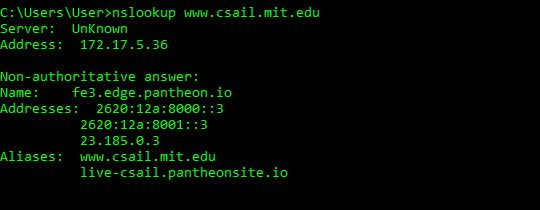
\includegraphics{DNS-via-nslookup.JPG}
\begin{enumerate}
    \item The request is for a DNS lookup of www.csail.mit.edu
    The address is 23.185.0.3\\
    Of note is the previous 2 addresses, which are 2620:12a:8000::3 and 2620:12a:8001::3\\
    Those are actually IPV6 addresses, which is a different protocol from what you're currently learning. Nevertheless it's an address too.
    \item The Address provider, is listed at the top. While it says Server: UnKnown, the IP address of your DNS server is clearly written there, which is 172.17.5.36
    \item Noteworthy is the answer is non-authoritative, because the answer is from your DNS server, not directly from the organisation's DNS server. Your DNS server is simply echoing it to you while caching it.
\end{enumerate}
\subsubsection{Mail server interaction}
If one wants to send a mail to someone say, bob@mit.edu, which IP address should he send mail to?\\
The answer is really to get a MX reply from the DNS of that organisation. To refresh your memory, the MX reply from a DNS server tells you two things: \textbf{16-bit preference and name of the host that acts as a mail exchange server for a domain}. This implies that we should send an inquiry to the mit DNS server for their mail servers.\\ 
However, to do this we cannot use nslookup. This is because nslookup is to look up a name server. Not to inquire something from the name server. To do this, we use a different tool, known as \textbf{dig}. 
\subparagraph{4.5.6.1 Dig tool\\} %there isn't subsubsubsection. so this will have to do.
The dig tool was developed for a different reason from nslookup. It is designed to send inquiries to DNS servers. In this case, we use it in the following fashion:\\
dig {address} {type}\\
this allows us to send a query of the MX type. to obtain the required mail servers. An example command is shown below:\\
\noindent\makebox[\textwidth]{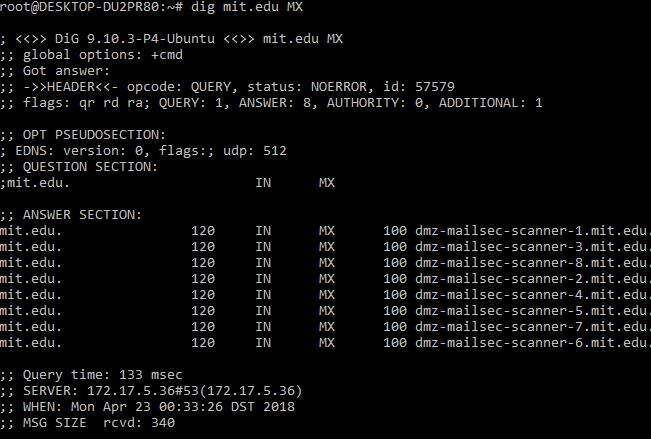
\includegraphics[]{dig-mit-edu.JPG}}
As seen, there are 8 mail servers that are available. This is due to the need to split the load between several servers and to maintain system integrity.\\
However, this does not include any authoritative answers.\\
So the difficulty in actually obtaining a authoritative answer is sometimes due to the intermediate DNS server/local DNS server caching the query, then echoing it back to you. As a result, we cannot always obtain an authoritative answer. Should you wish to \textbf{FORCE} an authoritative answer, the first thing you can do is use: \\
dig {site you wish to look up} {query type} +trace.\\
the +trace command forces the log of recursive commands to also be echoed to you, allowing you to find a possible authoritative name server. One such example is shown below:\\
\noindent\makebox[\textwidth]{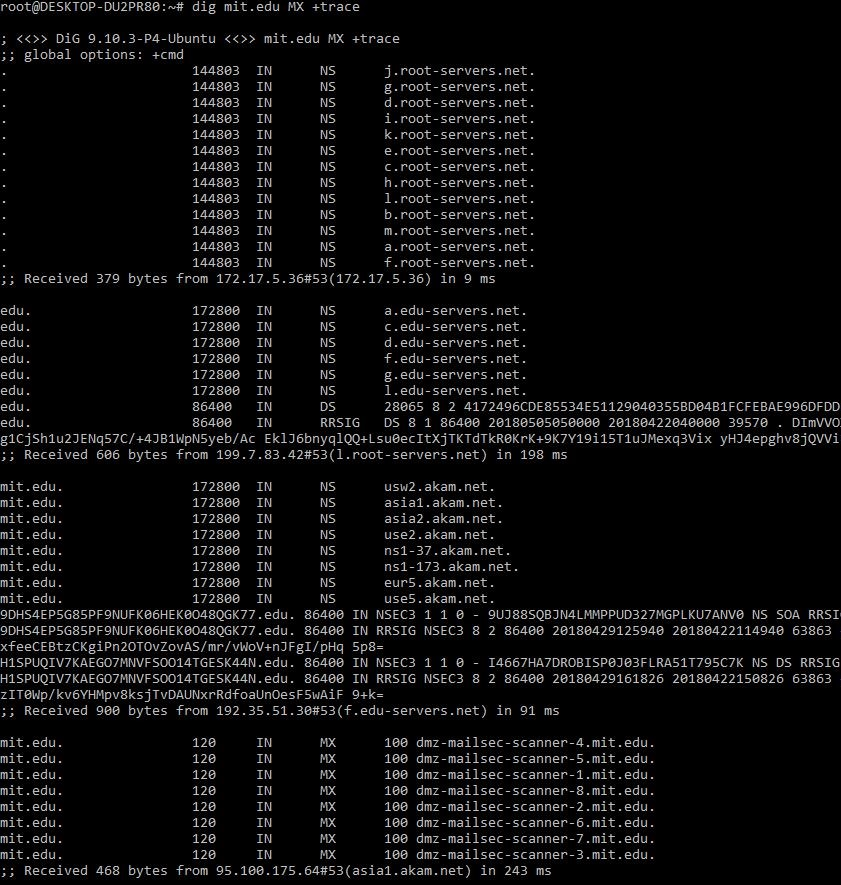
\includegraphics[width=\paperwidth]{digMX+trace2.jpg}}
Then looking at the final response, which states which DNS server it came from (in this case, asia1.akam.net), we are able to find a server that can possibly give authoritative answers.\\
After this, simply run another dig command:\\
dig {website} {query} @{Name server address}\\
this will enable you forcibly obtain an authoritative answer straight from the authoritative DNS server. Of note is that @{name server} allows you to basically query any dns server. An example output is below.\\
\noindent\makebox[\textwidth]{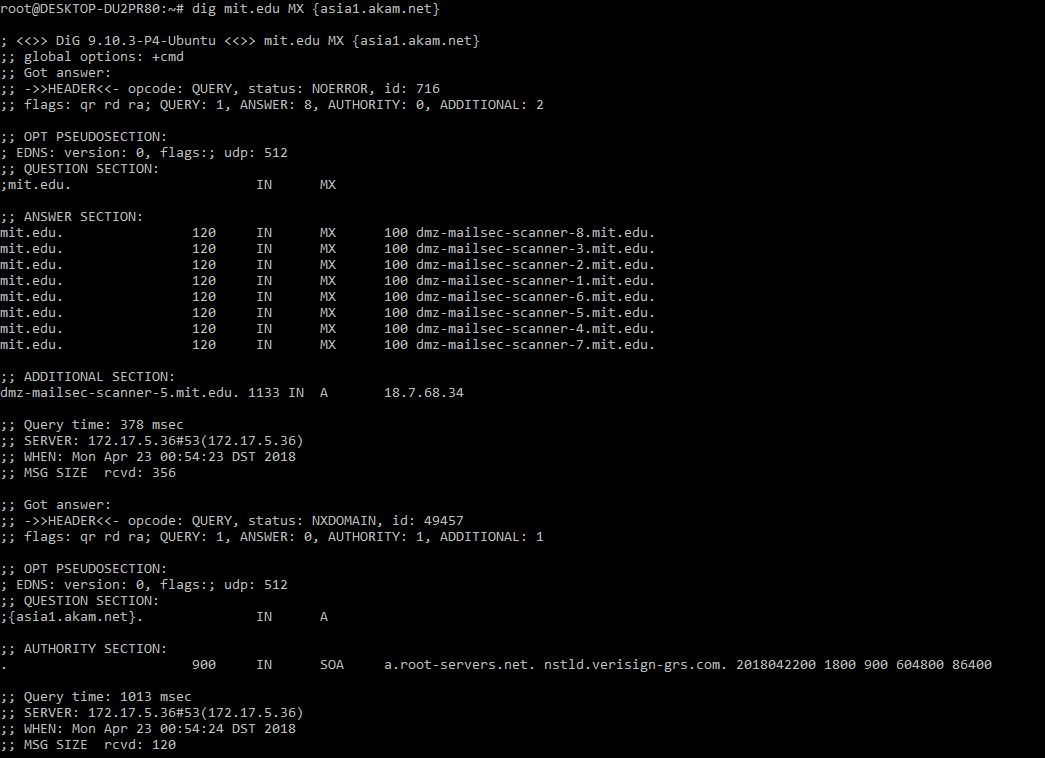
\includegraphics[width=\paperwidth]{dig-mit-edu-auth.JPG}}
Dig Answer Flag Examples:
\begin{itemize}
    \item QR specifies whether this message is a query (0), or a response (1)
    \item OPCODE A four bit field, only valid values: 0,1,2
    \item AA Authoritative Answer
    \item TC TrunCation (truncated due to length greater than that permitted on the transmission channel)
    \item RD Recursion Desired
    \item RA Recursion Available
    \item Z Reserved for future use. Must be zero
\end{itemize}

\pagebreak
\subsubsection{whois command}
The whois command is a protocol that is used for querying databases that store the registered users or assignees of an internet resource. This includes domain name, an IP address or other relevant information.\\
If you need to search for someone's IP, whois command can be used, if you have their namespace address.\\
\subsubsection{DNS Issues}
There is a cost on the indirection of DNS in general. Due to the spreading of servers, while we obtain general scalability portability and the ability to perform many-to-one mappings (aliasing), we compromise the security of the servers due to the possibility of posioning/intercepted mappings.\\
\subsection{Client-server and the Web: The application layer}
\subsubsection{Sockets}
While an IP address points you to the machine, but does not tell you the process you should be looking for.\\
Due to process ID being volatile and not meant for external usage to point to the correct process, we need another pointer, the socket.\\
Therefore, packet headers contain port numbers in order to tell the other computer which process it should look for.
\subsubsection{Multiplexing/Demultiplexing}
Multiplexing is the process of combining several analog or digital signals to be sent via one signal. Demultiplexing is the opposite process, where we split the multiplexed signal into several different signals again. It requires a multiplexer on one side and a demultiplexer on the receiving end. There are several ways to achieve this, and two of the covered ways are frequency division multiplexing where the spectrum of each input signal is shifted to different bands, and time division multiplexing, where signals take turns.\\
\paragraph{4.6.2.1 Connection-oriented (TCP) demultiplexing}
Essentially, in order to split the signals among one TCP connection, the packets sent contain a their source and destination IP address and port numbers, allowing for communication between two computer processes.\\
\paragraph{4.6.2.2 TCP Socket Programming}
\begin{itemize}
    \item The server has to be already running before the client contacts it. 
    \item The server must have a socket that welcomes client contact.
    \item The client contacts by creating a TCP socket with the IP address and port number of the server process.\\ Socket creation will establish a connection to the server.
    \item Servers will create a new socket for the server process to communicate with the client upon contact. Keep in mind that the server still has a separate server socket. \item The Source port numbers are used to distinguish the clients.
\end{itemize}
\paragraph{4.6.2.3 UDP Socket programming}
UDP has no "connection between the client and server. There is no handshake before sending data. The sender simply attaches the IP destination and port number. Of note is that it may be lost or received out of order. It provides unreliable transfer of groups of bytes.
\subsubsection{Web/HTTP Pages}
    HTTP stands for hypertext transfer protocol. \\
    HTTP itself is stateless and maintains no information about past client requests, unless cookies are used.\\
    The HTTP page itself that is transferred might contain further references to other servers to obtain more resources that the current services might not have.\\
    Currently there are 2 HTTP connection types. There is HTTP/1.0, non-persistent HTTP, and HTTP/1.1, persistent HTTP.
    \begin{itemize}
        \item non persistent HTTP, HTTP 1.0 allows only one object sent over TCP connections
        \item persistent HTTP, HTTP 1.1, the server leaves the connection open after sending the response, allowing for multiple objects to be sent over a single TCP connection.
    \end{itemize}
    The reason for using HTTP 1.1 connections as opposed to that of HTTP 1.0 is due to the number of round trip time packets take, the number of connections, and the allowance for instant requesting for objects.\\
    When using non-persistent HTTP, browsers will often parallel TCP connections to fetch the referenced objects.
\subsubsection{Spacetime diagram of sending 10 jpegs using persistent connection}
Use the following diagram as a guide on how to draw what they call a space-time diagram in this course. This image is that of a HTTP request scenario assuming persistent connection(HTTP 1.1) and pipelining.
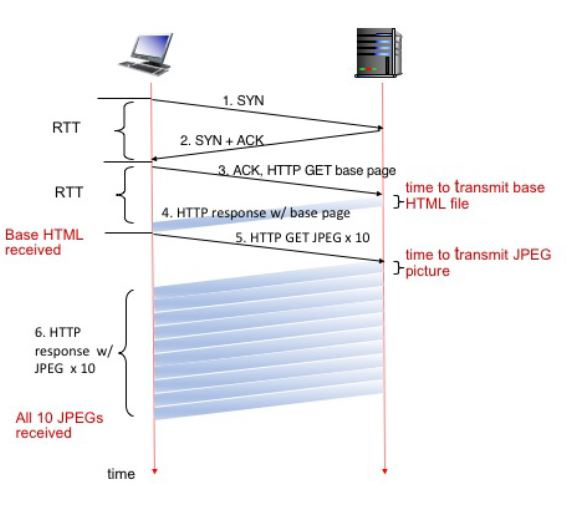
\includegraphics{Syn+AckSpacetimediagram.JPG}
\subsubsection{HTTP Request message format}
Depending on the type of request that is sent over, the actual contents and structure of the message will vary somewhat. \\
The general structure of the HTTP message is as follows:
\begin{itemize}
    \item Start line \\
    The message start line contains the Request  and  the Status Line. The request line is the request method that the client is using, and the status line is only included in the message is the sender was from a server.
    \item Header Fields\\
    The header fields will contain one of two things, depending if it is a message response or a request.
    \begin{itemize}
        \item If it was a request:\\
        It will contain fields that allow the client to pass additional information about the request and the client itself to the server. Example fields include: Accepted Charset, Accepted Encoding, Accepted Language, Expect, Authorization, From, Host, If-Match, If-Modified-Since, Range, Referer.
        \item If it was a response:\\
        It will contain response headers, such as: Accept-ranges, Age, Location, Server, WWW-authenticate.
    \end{itemize}
    \item The final part is the Message body. \\
    It is an optional part, and carries the request/response data that is required for the message.
\end{itemize}
Here are those HTTP requests that you'll have to know\\
\paragraph{4.6.5.1 HTTP 1.0 (non persistent)}
Request types:
\begin{enumerate}
    \item GET\\
    Request information from the server for retrieval.
    \item POST \\
    Request the server accept the fields of data stored inside the message body, possibly for processing or storage.
    \item HEAD\\
    Ask the server to leave requested object out of response
\end{enumerate}
\paragraph{4.6.5.2 HTTP 1.1 (persistent)}
Request types:
\begin{enumerate}
    \item GET
    \item POST
    \item HEAD
    \item PUT\\
    Upload the file in entity body to the path specified in the URL field.
    \item DELETE\\
    Deletes the file specified in the URL Field.
\end{enumerate}    
\subsubsection{Telnet (TCP)}
Telnet is a client-server protocol. Telnet enables you to open communications between a server and your computer (the client). As a result, you can also send HTTP POST and GET requests.
\subsubsection{HTTPS}
HTTPS Runs at port 443.\\
Uses (SSL) encrypted communications\\
\subsubsection{HTTP Response status codes}
The more well known codes you'll need to know are below:\\
\begin{enumerate}
    \item 200 OK - Request succeeded, requested object is in the message
    \item 301 Moved Permanently - Requested object is in a new location: and specified later in the message.
    \item 400 Bad Request - Request message is not understood by the server
    \item 404 Not found - the requested document is not found on this server
    \item 505 HTTP Version not supported
\end{enumerate}

\subsubsection{Cookies}
Cookies are arbitrary pieces of data, usually chosen and first sent by the web server, and stored on the client computer by the web browser. The browser then sends them back to the server with every request. They aid in maintaining state requests.\\
Cookies are composed of four components:\\
\begin{enumerate}
    \item Domain
    \item Path
    \item Expires
    \item Max-Age
\end{enumerate}
There are also two additional components: Secure and HttpOnly. However, they are optional fields and their presence simply indicates that they should only be treated as such.\\
Cookies can be used for authorization, Shopping carts, Recommendations, User Session State.
\subsubsection{Proxy Servers}
Proxy Servers are similar to a DNS server. The only difference is that they act as both client and server. Upon requesting a web page from a computer, the proxy server will check its cache for the webpage. Upon finding a hit, it immediately returns the webpage. But if it misses, it queries the relevant DNS servers, gets the webpage, stores it, and returns a copy to the original requester. Depending on the hit rate of the cache, this can heavily reduce the load on the external network link. This is known as a conditional GET. - If modified since - then send me a new one. else send me my 304 not modified header.


\end{document}